The current trend is to construct programs that play games with imperfect information, for instance Hanabi \cite{DBLP:journals/corr/abs-1902-00506}, but also video games such as Starcraft 2 \cite{DBLP:conf/ijcai/HuLLPX18} An important ingredient is to reason about higher-order knowledge (an agent knows that another agents knows that...). That is why we claim that epistemic logic and its dynamic extension, Dynamic epistemic logic (\cite{baltag1998logic}, \cite{DitmarschvdHoekKooi}), may offer a formal tool to provide explanation in such AI programs. needs to be understood is relevant in AI, especially in strategic reasoning \cite{DBLP:journals/ijgt/Aumann99}.

The only tool we are aware of that enables to see and explore mental states of agents is \emph{Hintikka's world} and was presented at ECAI-IJCAI 2018 \cite{DBLP:conf/ijcai/Schwarzentruber18}. 
\emph{Hintikka's world} is a proof of concept of a graphical user interface that represent Kripke models by  comic strips, as shown in Figure \ref{figure:gui}. The tool is available at the following address:
\url{http://hintikkasworld.irisa.fr/}. 


Kripke models are graphs and they were represented explicitly in memory in the first version of the tool. Explicit models are useful to learn how dynamic epistemic logic works by means of toy examples: muddy children, Sally and Anne  \cite{wimmer1983beliefs}, etc.  However, in real card games, such as Hanabi, there are .... possible configurations of cards. Thus, it is impossible to represent the full graph in memory:  the first version of Hintikka's world does not \emph{scale}. 

That is why, we proposed to represent Kripke models symbolically by means of Binary Decision Diagrams as it was done in the tool DEMO\footnote{The current implementation does not rely on DEMO since their work is not well-suited for a web application.}  \cite{DBLP:conf/lori/BenthemEGS15}. 





\begin{figure}
	\begin{center}
		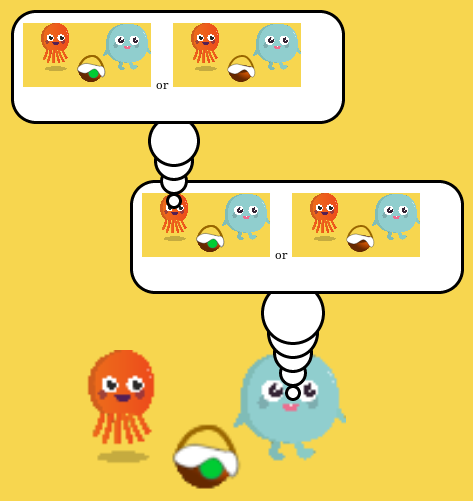
\includegraphics[width=4cm]{screenshot.png}
	\end{center}
	\caption{Graphical user interface of \emph{Hintikka's world}\label{figure:gui}}
\end{figure}
